\chapter{Introducción}
%TODO
% Importancia del trabajo en el contexto
% Propósito del trabajo
% Principales logros del trabajo
% Visión general del trabajo
% Síntesis y organización del documento


\section{Planteamiento del problema}
En la actualidad, la creciente contaminación acústica amerita la implementación de redes de monitoreo continuo de ruido
o mediciones puntuales empleando instrumentos adecuados (entre estos los sonómetros y calibradores acústicos), con el
propósito de cuantizar los niveles de ruido ambiental, de emisión de ruido de fuentes sonoras específicas y de
exposición sonora, para luego comparar con los niveles máximos permitidos por la normativa nacional e internacional
relacionada y tomar decisiones al respecto.
Para garantizar la confiabilidad de tales mediciones o asegurar la validez de sus resultados, en Colombia, entidades
como el Instituto de Hidrología, Meteorología y Estudios Ambientales (IDEAM) exigen que las organizaciones que prestan
estos servicios cuenten con sonómetros calibrados periódicamente bajo el estándar internacional
\mbox{IEC 61672--3}~\citeyearpar{IEC_TC29_2013_3}, y con calibradores acústicos calibrados periódicamente de acuerdo con
el estándar internacional \mbox{IEC 60942, Anexo B}~\citeyearpar{IEC_TC29_2017}, por parte de un organismo de evaluación
de la conformidad (OEC), en este caso un laboratorio de calibración acreditado por el Organismo Nacional de Acreditación
de Colombia (ONAC) en \mbox{ISO 17025}~\citeyearpar{ISO_CASCO_2017}, con el fin de verificar que estos instrumentos
continúan cumpliendo las especificaciones normalizadas según su clase.

Los calibradores acústicos normalmente son empleados como patrones de trabajo en las verificaciones de campo periódicas
de los sonómetros.
Para estos calibradores, el Anexo B de la norma \mbox{IEC 60942} establece tres pruebas que evalúan el funcionamiento
del calibrador en tres magnitudes:
1) Nivel de presión acústica,
2) frecuencia y
3) distorsión armónica más ruido (THD+N).

Por su parte, la norma \mbox{IEC 61672--3} describe una serie de pruebas acústicas y eléctricas que se realizan a
sonómetros integradores clase 1 y 2, cuyo propósito es comprobar el funcionamiento del sonómetro en:
1) La sensibilidad de su micrófono (para lo cual se usa un calibrador acústico calibrado previamente y que esté en
conformidad con las especificaciones de la \mbox{IEC 60942}).
2) Las redes de ponderación frecuencial A, C y Z. 3) Las ponderaciones temporales F (\emph{fast}) y S (\emph{slow}).
4) El rango lineal de niveles.
5) La medición de niveles promediados en el tiempo, niveles de exposición sonora y niveles pico.
6) La indicación de sobrecarga.
7) La exposición a largos periodos de medición y a niveles de sonido elevados.
Dicha comprobación se hace comparando con las especificaciones definidas en la norma \mbox{IEC 61672-1:2013}, según la
clase del sonómetro.

A continuación se presenta una revisión de los avances en el desarrollo de sistemas de calibración de sonómetros,
considerando especialmente su versatilidad (que el alcance de su aplicación abarque sonómetros de cualquier marca), su
actualidad (que siga los lineamientos de la última versión de la norma internacional), su funcionalidad (que ofrezca
herramientas útiles como procesamiento, análisis, almacenamiento y presentación de datos que faciliten la gestión
metrológica) y su costo.


\section{Antecedentes}

\subsection{Sistemas de calibración comerciales desarrollados por fabricantes}
\begin{figure}[!h]
    \caption{Estación de medición para la calibración de instrumentos acústicos de medida en el laboratorio AP146 en
    Polonia.}
    \label{fig:AP146Laboratory}
    \centering
    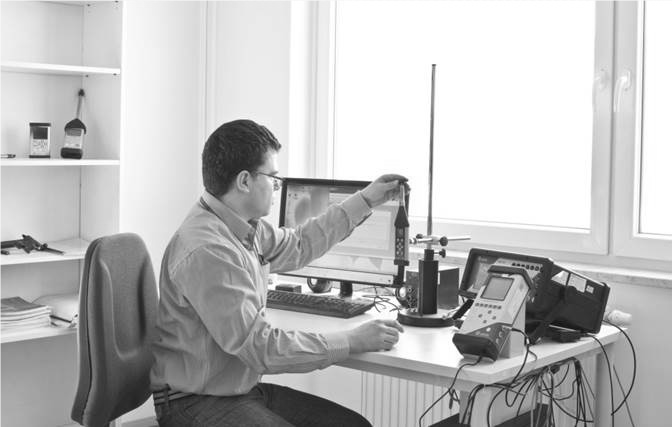
\includegraphics[width=0.8\textwidth]{1_Intro/AP146Laboratory}
    \caption*{\footnotesize Tomado de~\cite{Podgorski2016}}
\end{figure}

Es común encontrar que las organizaciones fabricantes de sonómetros adicionalmente presten servicios de calibración
acreditada (e.g.\ Svantek, Brüel \& Kjær y 01dB), por lo que prácticamente también se pueden denominar OEC\@.
Pero estos OEC en especial, tienen la posibilidad de implementar procedimientos automáticos de calibración sin
limitaciones, puesto que tienen acceso a los comandos de control específicos de sus modelos de sonómetros.
Un ejemplo de eso se encuentra en el artículo de~\cite{Podgorski2016}, en el que se hace una descripción del laboratorio
AP146 en Polonia que pertenece a Svantek y está acreditado por el Centro Polaco de Acreditación (PCA).
En ese artículo se presenta el desarrollo de un \emph{software} de calibración que han validado, desde el que se envían
instrucciones a los instrumentos que generan las señales y a los que las miden, también es posible generar
automáticamente reportes de resultados.
No obstante, sólo es posible usar este \emph{software} con los sonómetros que fabrica la compañía.
Para sonómetros de otras marcas las configuraciones deben hacerse manualmente y por ende el tiempo total de calibración
llega a ser por lo menos el doble.
La figura~\ref{fig:AP146Laboratory} muestra la estación de medición de este laboratorio.

\begin{figure}[!h]
    \caption{Sistema de calibración de sonómetros Type 3630-A desarrollado por Brüel \& Kjær.}
    \label{fig:BK3630A}
    \centering
    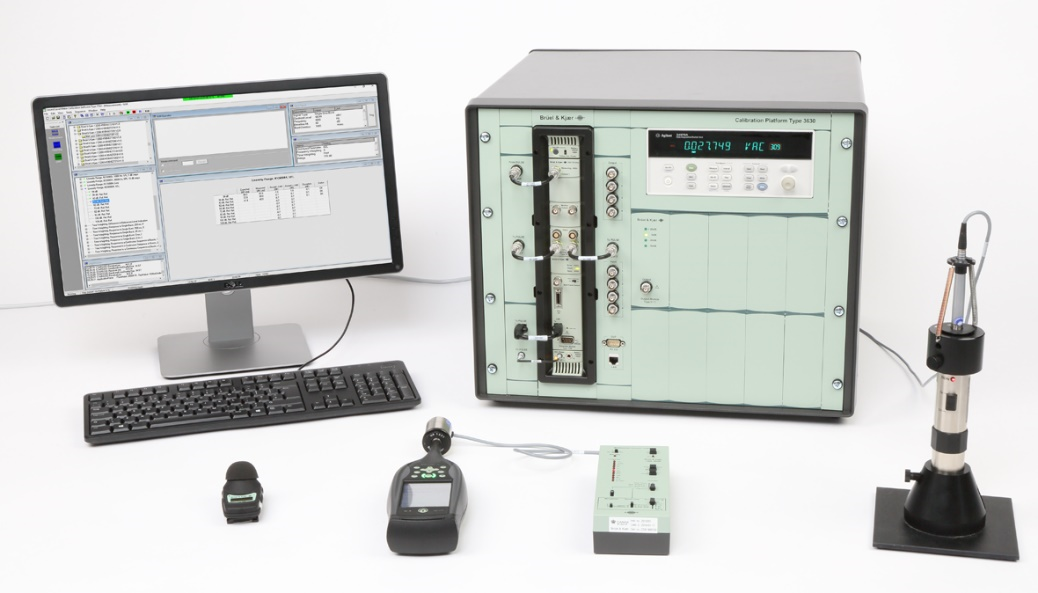
\includegraphics[width=0.8\textwidth]{1_Intro/BK3630A}
    \caption*{\footnotesize Tomado de~\cite{BruelKjaer2000}}
\end{figure}

La figura~\ref{fig:BK3630A} muestra el Type 3630-A, uno de los sistemas de calibración más completo y compacto.
Fue desarrollado por Brüel \& Kjær~\citeyearpar{BruelKjaer2000}, que permite la calibración periódica y la estimación
de incertidumbre de medida para sonómetros Brüel \& Kjær y también de otras marcas.
Además, ofrece la posibilidad de calibrar en modo automático (si el sonómetro dispone de una interfaz serial),
semiautomático (si el sonómetro tiene una salida análoga que corresponda satisfactoriamente con la indicación en
pantalla) y manual (si el sonómetro no cuenta con ninguna salida análoga), con secuencias predefinidas o personalizadas
por el usuario.
Tiene una base de datos de clientes e instrumentos integrada, lo que permite la trazabilidad de los intervalos de
calibración de los patrones de trabajo.
Es capaz de generar certificados de calibración con detallados reportes de resultados.
Permite calibrar dosímetros, calibradores acústicos y filtros.
Sin embargo, por defecto, únicamente tiene disponibles los ensayos de acuerdo con la norma \mbox{IEC 60651} y la
\mbox{IEC 60804}, que quedaron obsoletas rápidamente con el avance tecnológico~\citep{Beyers2014}.
Los ensayos de acuerdo con la \mbox{IEC 61672--3} están disponibles sólo como complementos que el usuario debe comprar.

\subsection{Sistemas de calibración desarrollados por otras organizaciones}
Los anteriores sistemas de calibración desarrollados por los fabricantes más prominentes son sofisticados y costosos,
por lo que los demás OEC, que en su mayoría son organizaciones independientes, deben implementar su propia estación de
trabajo y desarrollar su propio procedimiento de calibración.
El hecho que se desconozca la codificación de control del sonómetro propia de cada fabricante sugiere que lo más seguro
es que este procedimiento sea manual.

Para abordar esta problemática, hay un avance en la automatización del procedimiento de calibración, extendiendo el
alcance a cualquier sonómetro sin importar su modelo o marca, este es el trabajo realizado por~\cite{Zhong2010},
en el que desarrollaron un sistema de calibración implementando reconocimiento de imágenes.
De modo que el resultado es obtenido automáticamente de la indicación en la pantalla del sonómetro, superando así la
limitación más común en los sistemas automáticos de calibración de los fabricantes.
Tal funcionamiento hace de este un sistema mucho más versátil, con el que igualmente se pueden generar de forma
automática los reportes con los resultados de calibración.
Sin embargo, dada su fecha de publicación (2010), está basado en la versión anterior de la
\mbox{IEC 61672--3}~\citeyearpar{IEC_TC29_2013_3}.
Y, por otro lado, utiliza un método de calibración distinto, en el que se requiere una cámara anecóica para calibrar en
campo libre las frecuencias de $\qty{500}{\Hz}$ a $\qty{20}{\kHz}$, un acoplador activo para calibrar en campo de
presión las frecuencias de $\qty{10}{\Hz}$ a $\qty{500}{\Hz}$ y un micrófono patrón de laboratorio para obtener las
respuestas de referencia de los campos, lo que eleva el costo.

La anterior revisión de sistemas de calibración desarrollados por fabricantes y por otros laboratorios indica que hace
falta un sistema de calibración de sonómetros actualizado, versátil, y de bajo costo, pero que no comprometa los
resultados.
Es en esa vía que se planteó este trabajo y se da cumplimiento a los siguientes objetivos.


\section{Objetivos}

\textbf{General}

Desarrollar un sistema de calibración periódica de sonómetros y calibradores acústicos de conformidad con las normas
\mbox{IEC 61672-3:2013} e {IEC 60942:2017}.
\vfill
\pagebreak

\textbf{Específicos}

\begin{enumerate}
    \item Formular un modelo en GRAFCET como base para el desarrollo de un sistema de calibración periódica de
    calibradores acústicos.
    \item Implementar las secuencias de comando (a través de bus GPIB) para configurar parámetros de señal y, a su vez,
    recibir resultados de los instrumentos de medición.
    \item Desarrollar un método de reconocimiento de imágenes para detectar los niveles instantáneos ponderados en
    tiempo y en frecuencia desde la pantalla del sonómetro.
    \item Desarrollar un método que permita tener en cuenta la variabilidad de los niveles en pantalla instantáneos
    ponderados en tiempo y en frecuencia del objetivo 3, (mediante mediciones de larga duración), para la estimación
    del mesurando y de la incertidumbre de medición.
\end{enumerate}

\subsection{Alcance de los objetivos}
El sistema de calibración se implementó para ejecutar las pruebas de calibración de los numerales 9.3 (apoyado en la
IEC 60942), 13, 14 y 16 de la \mbox{IEC 61672--3}.
Los indicadores de interés son los niveles instantáneos con ponderación temporal (\emph{slow} o \emph{fast}) y
ponderación frecuencial ($A$, $C$, o $Z$), i.e. $L_{AF}$,$L_{AS}$,$L_{CF}$,$L_{CS}$,$L_{ZF}$ o $L_{ZS}$, dependiendo
de la prueba y según estén disponibles en el sonómetro sujetos al periodo de actualización de la pantalla del sonómetro.


\section{Estructura del documento}
Antes de introducir el desarrollo técnico de los objetivos, este documento inicia con un capítulo de metodología e
instrumentación en el que se describen el marco normativo y los equipos utilizados en el sistema desarrollado.
Luego, en cumplimiento del tercer objetivo, el capítulo dos explica el diseño e implementación del algoritmo
para el reconocimiento de los caracteres numéricos que representan los niveles de sonido mostrados en la pantalla del
sonómetro.
En el capítulo cuatro se presenta el GRAFCET del objetivo uno y los detalles de implementación del objetivo dos en las
aplicaciones desarrolladas en Python.
En el último capítulo se explican las consideraciones teóricas-experimentales que forman el punto de partida del método
del cuarto objetivo.
Asimismo, se incluye el marco teórico de las cadenas de Markov que son la herramienta esencial del
método y se expone un resultado de ejemplo.
Finalmente, se concluye el documento con una revisión del trabajo realizado y sugerencias para desarrollo futuro.